\chapter{Fundamentação Teórica}
\label{cap:fundamentacao}

Este capítulo contextualiza os desafios do ensino de programação e introduz o conceito de \textit{logging} como uma prática crucial da Engenharia de Software. Em seguida, explora o uso de \textit{logs} no contexto educacional, detalha a taxonomia de conceitos relacionados e descreve a extensão LOGADO, contribuição prática deste trabalho, bem como a Design Science Research como abordagem metodológica adotada.

\section{Desafios no Ensino de Programação e a Lacuna Instrucional sobre Logging}
\label{sec:desafios-lacuna}

O ensino de programação vai além da transmissão de conhecimentos técnicos, abrangendo boas práticas de desenvolvimento, integridade acadêmica e a compreensão do ciclo de vida do software. No entanto, a literatura pedagógica apresenta uma lacuna significativa nesse aspecto.

O mapeamento do estado da arte, realizado por meio de uma revisão sistemática de livros-texto fundamentais, evidencia essa lacuna. Obras amplamente adotadas internacionalmente, como as de \citet{pressman2020} e \citet{sommerville2016}, e, no contexto nacional, \textit{Engenharia de Software Moderna} \citet{valente2020}, dedicam capítulos substanciais a temas como testes e qualidade de software. Nenhuma delas, porém, aborda o \textit{logging} de forma pedagógica e estruturada, como uma prática de engenharia com estratégias e boas práticas específicas, o que está alinhado com observações da literatura recente \cite{gu2022logging}.

\subsection{Pesquisas sobre Logs no Ensino de Programação no Brasil}

Diante da lacuna identificada, este trabalho busca reforçar o potencial pedagógico dos rastros digitais no ensino de programação. Para fundamentar essa proposta, foi conduzida uma busca sistemática no Portal da Sociedade Brasileira de Computação (SBC) com a string \texttt{"log"~ OR "logging"~ AND "ensino de programação"}, que retornou um número insignificante de trabalhos, conforme detalhado na Tabela \ref{tab:repositorios} (Apêndice A).

\section{Logging: Conceitos e Aplicações na Engenharia de Software}
\label{sec:conceitos-logging}

As práticas de registro de rastros em sistemas computacionais abrangem diversos conceitos. Como exemplo, a taxonomia de \cite{gu2022logging} define os seguintes elementos fundamentais\footnote{Os termos originais em inglês foram mantidos por serem amplamente utilizados na literatura da área de Engenharia de Software e não terem tradução consagrada no português técnico.}:

\begingroup
\renewcommand{\arraystretch}{1.2}
\begin{tabular}{p{0.3\textwidth}p{0.3\textwidth}p{0.3\textwidth}}
    \texttt{Log statement} & \texttt{Log message} & \texttt{Log} \\
    \texttt{Log level} & \texttt{Log content} & \texttt{Log location} \\
    \texttt{Log placement} & \texttt{Logging} & \texttt{Logging practice} \\
\end{tabular}
\endgroup
\vspace{2em}

Para os fins desta pesquisa, não é necessário aprofundar cada um desses termos; interessa prioritariamente a distinção entre \textit{log} (registro completo) e \textit{log message} (entrada individual), conforme adotado adiante.

Neste trabalho, \textit{log} refere-se ao registro completo das atividades do sistema, enquanto \textit{log message} compreende entradas individuais com marcação temporal que representam eventos específicos durante o desenvolvimento de código.

Segundo \cite{rice1983use}, o monitoramento de sistemas pode ser entendido como um registro automático de transações. A importância dos \textit{logs} é vasta, sendo utilizados em tarefas como detecção de anomalias, depuração, diagnóstico de desempenho e modelagem de comportamento de sistemas \cite{fu_where_2014}. Estudos como o de \cite{yang2021interview} confirmam que os desenvolvedores os utilizam primariamente para análise de problemas, buscando informações como a propagação de erros, \textit{timestamps} e o \textit{dataflow} entre componentes.

\section{A Análise de Logs como Ferramenta Educacional}
\label{sec:logs-educacionais}

A aplicação de análise de \textit{logs} no ensino de programação representa uma transposição dessa prática da Engenharia de Software para a avaliação do processo de aprendizagem. Para que essa análise seja viável, é necessário um mecanismo de captura dos rastros gerados durante a atividade. A Figura \ref{fig:fluxograma-logado} ilustra esse modelo conceitual de coleta.

\begin{figure}[h]
\centering

\includegraphics[width=0.85\textwidth]{fluxograma-logado.png}
\caption{Modelo de coleta de dados educacionais durante a atividade de codificação. O plugin LOGADO monitora o processo, gerando logs que registram a jornada do aprendiz, em contraste com o artefato final (código) que é o foco da avaliação tradicional.}
\label{fig:fluxograma-logado}
\end{figure}

A Tabela \ref{tab:comparacao-avaliacao} contrasta a abordagem tradicional com a proposta deste trabalho:

\begin{table}[h]
\centering
\caption{Comparação entre abordagens de avaliação em programação}
\label{tab:comparacao-avaliacao}
\begin{tabular}{p{0.45\textwidth}p{0.45\textwidth}}
\hline
\textbf{Avaliação Tradicional} & \textbf{Avaliação com Análise de \textit{Logs}} \\
\hline
Foca no produto final (código) & Foca no processo de desenvolvimento \\
Analisa o que foi produzido & Analisa como foi produzido \\
Avaliação predominantemente quantitativa & Inclui dimensões qualitativas do aprendizado \\
Visão estática do conhecimento & Visão dinâmica da curva de aprendizagem \\
Foco no indivíduo & Permite análise individual e em grupo \\
\hline
\end{tabular}
\end{table}

Enquanto a avaliação tradicional concentra-se na lógica, sintaxe e funcionalidade do código entregue, a análise de \textit{logs} captura os rastros digitais do desenvolvimento, revelando padrões de raciocínio, dificuldades específicas e estratégias de resolução de problemas.

Como sugerido por \cite{silva2022previsao}, variáveis preditoras podem ser extraídas diretamente do código-fonte, tais como: número de linhas lógicas, uso de estruturas de repetição, quantidade de identificadores e funções utilizadas. Esta abordagem alinha-se com a \textit{Learning Analytics}, que visa melhorar a qualidade do ensino e da aprendizagem por meio da análise de dados sobre o comportamento dos estudantes \cite{huang2020predicting}. Os \textit{logs} de programação funcionam, assim, como registros de aprendizagem (\textit{learning records}), revelando a experiência pessoal e as reflexões do estudante durante o processo de desenvolvimento \cite{du2005learning}.

\section{Design Science Research}
\label{sec:design-science-research}

Esta pesquisa adota a Design Science Research (DSR) como abordagem metodológica, amplamente utilizada em Computação para orientar o desenvolvimento de soluções tecnológicas voltadas a problemas práticos \cite{hevner2004design, peffers2007design}.

Diferentemente de pesquisas que apenas descrevem ou explicam fenômenos, a DSR concentra-se na criação de algo novo, um artefato, que atenda a uma necessidade real. No caso deste trabalho, o artefato é a extensão LOGADO para o Visual Studio Code.

Hevner et al. \cite{hevner2004design} estabelecem que pesquisas em DSR devem:
\begin{itemize}
    \item produzir um artefato útil;
    \item endereçar um problema relevante;
    \item avaliar rigorosamente o que foi construído;
    \item comunicar claramente os resultados.
\end{itemize}

Peffers et al. \cite{peffers2007design} propõem um processo prático em seis etapas: identificar o problema, definir os objetivos da solução, projetar e desenvolver o artefato, demonstrar seu uso, avaliá-lo e comunicar os resultados.

Este trabalho seguiu essas etapas. O problema identificado foi a falta de ferramentas de telemetria educacional no ensino de programação, para o qual se desenvolveu a extensão LOGADO. A avaliação ocorreu por meio da coleta e análise de logs gerados por estudantes em situação real de aula. Os resultados são apresentados e discutidos ao longo da dissertação, em especial nos Capítulos \ref{cap-resultados-discussoes} e \ref{cap-consideracoes-finais}.

\section{A Extensão LOGADO: Proposta de Implementação}
\label{sec:extensao-logado}

A extensão LOGADO foi desenvolvida para coletar rastros de aprendizagem nas disciplinas de programação que usam JavaScript como linguagem e tem o Visual Studio Code (VS Code) como editor principal, que é amplamente adotado no contexto educacional por sua leveza, gratuidade e suporte a extensões. A ferramenta captura, de forma transparente e não intrusiva, as palavras reservadas digitadas pelos estudantes durante a resolução de problemas de programação, registrando eventos de edição e gerando arquivos de log no formato JSON.

\subsection{Estado atual da implementação}

Atualmente, a extensão LOGADO encontra-se na versão \texttt{0.0.5} e está disponível para instalação no Visual Studio Code por meio do arquivo \texttt{.vsix}, acessível através da paleta de comandos da IDE. O código-fonte completo, a documentação e as instruções de instalação estão disponíveis publicamente no repositório GitHub do projeto\footnote{\url{https://github.com/gilmargn/logado-utfpr-ifam}}.

\begin{figure}[H]
    \centering
    \begin{minipage}{0.3\textwidth}
        \centering
        
\includegraphics[width=\textwidth]{../figuras/logado-icon.png}
        \caption{Ícone da extensão LOGADO}
        \label{fig:icone-logado}
    \end{minipage}
    \hfill
    \begin{minipage}{0.65\textwidth}
        \centering
        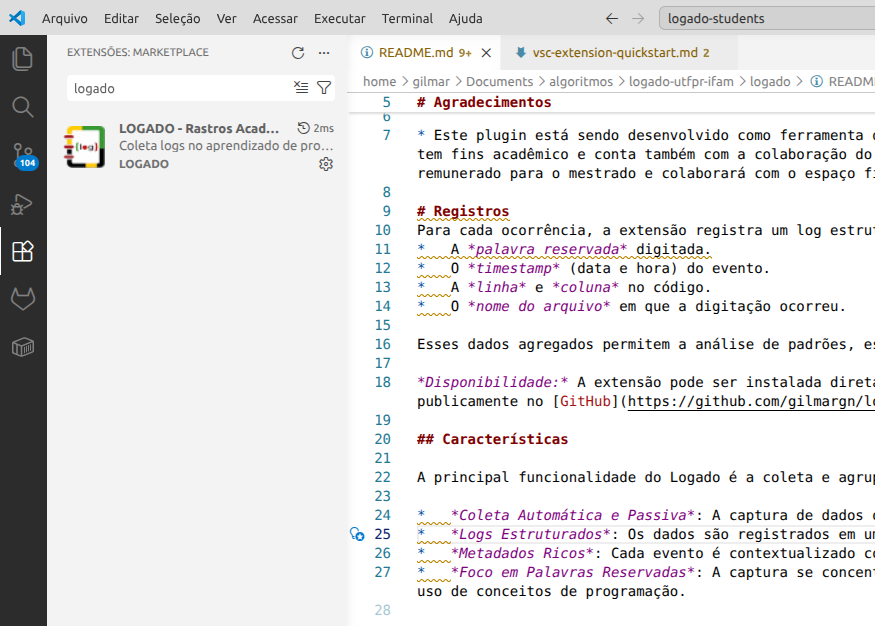
\includegraphics[width=\textwidth]{../figuras/vscode-logado.png}
        \caption{Visual Studio Code com a extensão LOGADO instalada}
        \label{fig:vs-code-logado}
    \end{minipage}
\end{figure}

A extensão opera em segundo plano, não requerendo configuração adicional. Uma vez instalada, a coleta de logs registra as palavras reservadas utilizadas, os respectivos \textit{timestamps} e a localização no código (arquivo, linha e coluna). O código é disponibilizado sob licença \textit{MIT}\footnote{Licença permissiva que permite reuso, modificação e distribuição, desde que mantido o aviso de direitos autorais.}, em consonância com os princípios da ciência aberta.

\subsection{Funcionalidades Principais}

A extensão LOGADO foi projetada para ser uma ferramenta leve e integrada ao fluxo natural do estudante, operando de forma transparente, mas nunca oculta.

\begin{itemize}
    \item Transparência: o estudante sabe exatamente quais informações são coletadas (palavras-chave, timestamp, arquivo, linha e coluna), não havendo coleta oculta de dados. Os logs são salvos em arquivos \texttt{.json} visíveis no explorador do VS Code.

    \item Gerenciamento de privacidade: a extensão opera em modo estritamente local. Os dados não são transmitidos para servidores externos sem consentimento explícito.

    \item Exportação de dados: os logs em JSON são salvos concomitantemente aos arquivos \texttt{.js}, podendo ser exportados para repositórios e compartilhados com pesquisadores ou instrutores.
\end{itemize}

\subsection{Arquitetura e Armazenamento de Dados}

A extensão foi desenvolvida em TypeScript, utilizando a API oficial do Visual Studio Code, com base na documentação oficial e em exemplos disponibilizados pela Microsoft. O trabalho consistiu em adaptar e aplicar os recursos existentes para a finalidade específica de coleta de logs educacionais.

O diferencial desta pesquisa não reside no código da extensão em si, mas na abordagem (telemetria de palavras reservadas como ferramenta pedagógica) e na aplicação (coleta de logs em contexto real de sala de aula). Os eventos capturados são salvos no formato JSON e armazenados localmente em arquivos de log, contendo palavra reservada, \textit{timestamp}, arquivo, linha e coluna.

A extensão não realiza análises automáticas sobre os dados coletados. Sua função limita-se à captura e ao armazenamento estruturado dos rastros, cabendo a pesquisas futuras aprofundar a análise desses registros.

\subsection{Notificação de Ativação}

Ao iniciar o VS Code com a extensão LOGADO instalada, uma notificação visual é exibida no canto inferior direito da tela (Figura \ref{fig:notificacao-logado}), informando ao estudante que os logs estão sendo coletados, em respeito aos princípios éticos de consentimento informado.

\begin{figure}[H]
    \centering
    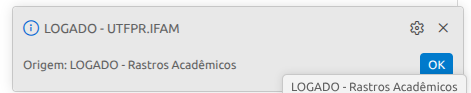
\includegraphics[width=0.85\textwidth]{../figuras/notificacoes-logado.png}
    \caption{Notificação exibida pela extensão LOGADO ao ser ativada}
    \label{fig:notificacao-logado}
\end{figure}

\subsection{Geração de Logs}

Para cada arquivo JavaScript editado, a extensão gera automaticamente um arquivo de log homônimo no formato JSON (\texttt{.json}), salvo no mesmo diretório do código-fonte. A Figura \ref{fig:logado-explorer} ilustra essa correspondência.

\begin{figure}[H]
    \centering
    
\includegraphics[width=0.85\textwidth]{data-structure.png} 
    \caption{Arquivos de log (\texttt{.json}) gerados para cada arquivo JavaScript}
    \label{fig:logado-explorer}
\end{figure}

No exemplo apresentado, é possível observar a estrutura adotada durante as atividades da disciplina de Estrutura de Dados: os arquivos \texttt{lista.js}, \texttt{fila.js} e \texttt{pilha.js} representam as implementações solicitadas, enquanto os arquivos \texttt{lista.json}, \texttt{fila.json} e \texttt{pilha.json} armazenam os logs de palavras reservadas gerados durante a digitação de cada algoritmo. Essa separação preserva o código original do estudante e mantém os dados organizados, facilitando etapas posteriores de pré-processamento e agrupamento.

Para ilustrar a aplicação prática, considere o desenvolvimento do algoritmo de cálculo de impressão apresentado na Listagem \ref{lst:algoritmo-impressao-js}. Durante sua implementação, a extensão LOGADO captura o uso de elementos da linguagem, gerando os registros estruturados apresentados na Listagem \ref{lst:algoritmo-impressao-json}.

\begin{figure}[H]
    \centering
    \begin{minipage}{0.48\textwidth}
        \centering
        \begin{lstlisting}[style=jsonstyle, caption={Algoritmo de cálculo de impressão - exemplo didático}, label={lst:algoritmo-impressao-js}]
let numero_paginas = parseInt(prompt("Número de páginas"))
let tipo_impressao = prompt("Tipo de Impressão\n0 - Frente e verso\n1 - Frente")

let valor = 0

if(tipo_impressao=='0'){
    valor = numero_paginas * 0.10
    document.writeln(`Páginas impressas: ${numero_paginas}<br> Valor final: R$ ${valor.toFixed(2)}`)
}
else{
    valor = numero_paginas * 0.15
    document.writeln(`Páginas impressas: ${numero_paginas}<br> Valor final: R$ ${valor.toFixed(2)}`)
}
        \end{lstlisting}
    \end{minipage}
    \hfill
    \begin{minipage}{0.48\textwidth}
        \centering
        \begin{lstlisting}[style=jsonstyle, caption={Exemplo de saída da extensão LOGADO}, label={lst:algoritmo-impressao-json}]
[
  {
    "keyword": "let",
    "timestamp": "2026-02-24 19:21:45",
    "file": "impressao.js",
    "line": 1,
    "column": 1
  },
  {
    "keyword": "parseInt",
    "timestamp": "2026-02-24 19:21:47",
    "file": "impressao.js",
    "line": 1,
    "column": 18
  },
  {
    "keyword": "prompt",
    "timestamp": "2026-02-24 19:21:48",
    "file": "impressao.js",
    "line": 1,
    "column": 28
  }
]
        \end{lstlisting}
    \end{minipage}
\end{figure}

